\begin{refsection}

\chapter{Pb--Pb and Th--Pb}
\label{ch:ThPbPb-R}

\section{Pb--Pb}\label{sec:PbPb-R}

\noindent\begin{minipage}[t]{.3\linewidth}
\strut\vspace*{-\baselineskip}\newline
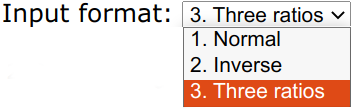
\includegraphics[width=\linewidth]{../figures/PbPbFormats.png}
\end{minipage}
\begin{minipage}[t]{.7\textwidth}
  \texttt{IsoplotR} accommodates three Pb--Pb formats. See
  Section~\ref{sec:PbPb} for details.
\end{minipage}

\begin{console}
PbPb <- read.data('PbPb3.csv',method='Pb-Pb',format=3)
\end{console}

\noindent\begin{minipage}[t]{.15\linewidth}
\strut\vspace*{-\baselineskip}\newline
\includegraphics[width=\linewidth]{../figures/PbPbPlotdevices.png}\\
\end{minipage}
\begin{minipage}[t]{.85\textwidth}
  Pb--Pb data can be visualised on five different plot devices.
  Additionally, the single aliquot age estimates can also be reported
  in a downloadable data table.
\end{minipage}

\noindent\begin{minipage}[t]{.6\linewidth}
\strut\vspace*{-\baselineskip}\newline
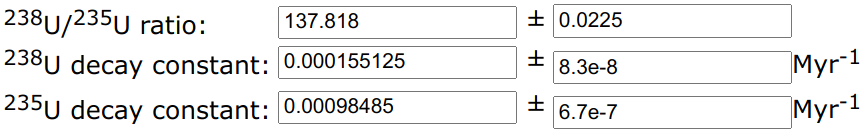
\includegraphics[width=\linewidth]{../figures/PbPbLambda.png}
\end{minipage}
\begin{minipage}[t]{.4\linewidth}
  The default \textsuperscript{238}U/\textsuperscript{235}U ratio is
  given by \citet{hiess2012}, and the U decay constants by
  \citet{jaffey1971}. These values can be changed here.
\end{minipage}

\begin{script}
# use the Steiger and Jaeger (1977) value with zero uncertainty
settings('iratio','U238U235',137.88,0)
# use the Schoene et al. (2006) value and uncertainty
settings('lambda','U238',0.000154993,0.00000013) 
\end{script}

\section{Isochrons}

\begin{enumerate}

\item \texttt{IsoplotR} offers the same three options to deal with the
  scatter of the data around the best-fit isochron line as the generic
  regression function of Section~\ref{sec:OtherRegression}.

\noindent\begin{minipage}[t]{.45\linewidth}
\strut\vspace*{-\baselineskip}\newline
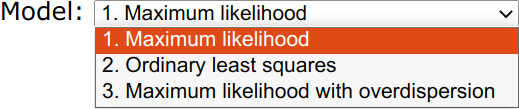
\includegraphics[width=\linewidth]{../figures/PbPbIsochronModels.png}
\end{minipage}
\begin{minipage}[t]{.55\linewidth}
  These three models represent three different ways to capture any
  excess dispersion of the data relative to the nominal uncertainties
  (Figure~\ref{fig:isochronMSWD}).
\end{minipage}

\begin{console}
isochron(PbPb,model=1)
\end{console}

\item Data can be fitted using conventional
  (\textsuperscript{207}Pb/\textsuperscript{204}Pb
  vs. \textsuperscript{206}Pb/\textsuperscript{204}Pb) or
  (\textsuperscript{207}Pb/\textsuperscript{206}Pb
  vs. \textsuperscript{204}Pb/\textsuperscript{206}Pb) isochrons
  (Section~\ref{sec:inverseIsochrons}).

  \noindent\begin{minipage}[t]{.22\linewidth}
\strut\vspace*{-\baselineskip}\newline

\includegraphics[width=\linewidth]{../figures/PbPbisochronInverse.png}
\end{minipage}
\begin{minipage}[t]{.78\linewidth}
  These two types of isochron yield similar ages provided that the
  uncertainties are relatively small compared to the isotopic ratio
  values.
\end{minipage}

\begin{console}
isochron(PbPb,inverse=TRUE)
\end{console}

\item As discussed in Section~\ref{sec:SKgrowth}, the mantle evolution
  model of \citet{stacey1975} can be included with the isochron plot.
  Any intersection(s) of the isochron with the mantle evolution curve
  is/are reported in the plot legend.

\noindent\begin{minipage}[t]{.45\linewidth}
\strut\vspace*{-\baselineskip}\newline

\includegraphics[width=\linewidth]{../figures/PbPbIsochronSKcurve.png}
\end{minipage}
\begin{minipage}[t]{.55\linewidth}
  The Stacey-Kramers curve may not be easy to spot for very radiogenic
  samples.
\end{minipage}

\item The appearance and numerical behaviour of Pb--Pb isochrons can
  be modified using similar options as the U--Pb isochrons of
  Section~\ref{sec:UPb-isochron-R}, and the general regression of
  Section~\ref{sec:OtherRegression}.

\noindent\begin{minipage}[t]{.4\linewidth}
\strut\vspace*{-\baselineskip}\newline
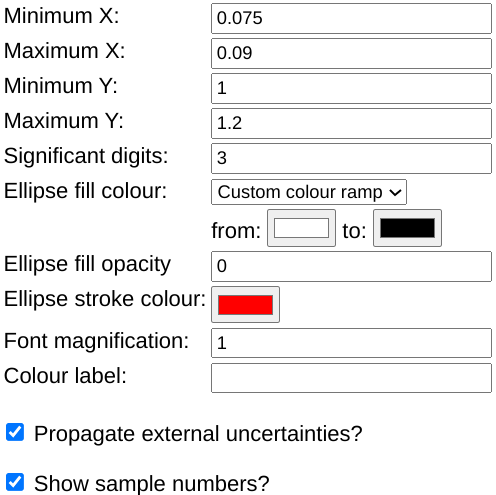
\includegraphics[width=\linewidth]{../figures/PbPbIsochronOtherOptions.png}
\end{minipage}
\begin{minipage}[t]{.6\linewidth}
  Tick the checkbox to propagate decay constant uncertainties
  (\texttt{exterr}) and label the error ellipses with the row numbers
  of the input data (\texttt{show.numbers}), use the textboxes to set
  the axis limits (\texttt{xlim} and \texttt{ylim}), significance
  level (\texttt{alpha}), significant digits (\texttt{sigdig}), the
  fill and stroke colour of the error ellipses (\texttt{ellipse.fill}
  and \texttt{ellipse.stroke}), font size (\texttt{cex}) and colour
  legend (\texttt{levels} and \texttt{clabel}).  
\end{minipage}

\begin{script}
isochron(PbPb,exterr=TRUE,show.numbers=TRUE,xlim=c(0,0.03),ylim=c(0,0.75),
         alpha=0.01,sigdig=3,ellipse.fill=NA,ellipse.stroke="red")
\end{script}
  
\end{enumerate}

\section{Ages}\label{sec:PbPbAges}

Although, as discussed in Section~\ref{sec:ThPbPbradial}, Pb--Pb ages
are usually calculated by isochron regression, it is also possible to
calculate the ages of each individual aliquots. Once these have been
calculated, it is then straightforward to turn them into the radial,
weighted mean, KDE and CAD plots. Thus, it is useful to introduce
\texttt{IsoplotR}'s age calculation function before discussing the
aforementioned plots.

\begin{enumerate}

\item In contrast with the U--Pb method, in which common-Pb correction
  often does not affect the age much, this correction is crucial for
  single grain Pb--Pb dating.
  
\noindent\begin{minipage}[t]{.35\linewidth}
\strut\vspace*{-\baselineskip}\newline
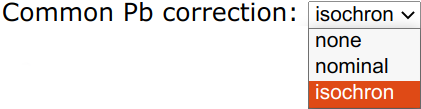
\includegraphics[width=\linewidth]{../figures/PbPbRadialPb0.png}
\end{minipage}
\begin{minipage}[t]{.65\linewidth}
  In contrast with the U--Pb data of Section~\ref{sec:UPbRadial}, the
  common Pb correction of Pb--Pb data is limited to two options:
  nominal and isochron. These implement the two procedures shown in
  Figure~\ref{fig:ThPbSingleGrain}.
\end{minipage}

\begin{console}
age(PbPb,common.Pb=2)
\end{console}

\item Nominal common Pb correction proceeds like the nominal common Pb
  correction of U--Pb data formats 4--6 (Section~\ref{sec:general}).

\noindent\begin{minipage}[t]{.4\linewidth}
\strut\vspace*{-\baselineskip}\newline
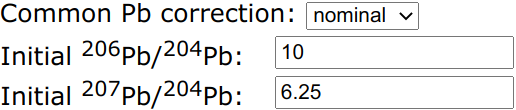
\includegraphics[width=\linewidth]{../figures/PbPbnominalPb0.png}
\end{minipage}
\begin{minipage}[t]{.6\linewidth}
  The nominal \textsuperscript{207}Pb/\textsuperscript{204}Pb and
  \textsuperscript{206}Pb/\textsuperscript{204}Pb ratios in this
  example correspond to a
  \textsuperscript{207}Pb/\textsuperscript{206}Pb ratio of 0.625,
  which equals the y-intercept of the inverse isochron.
\end{minipage}

\begin{console}
settings('iratio','Pb207Pb204',6.25)
settings('iratio','Pb206Pb204',10)
age(PbPb,common.Pb=1)
\end{console}

\item After possible common Pb correction, the resulting Pb--Pb ages
  are treated in exactly the same way as the U--Pb data of
  Section~\ref{sec:UPbRadial} and the generic data of
  Section~\ref{sec:OtherRadial}.

\end{enumerate}

\section{Th--Pb}\label{sec:ThPb-R}

\noindent\begin{minipage}[t]{.3\linewidth}
\strut\vspace*{-\baselineskip}\newline
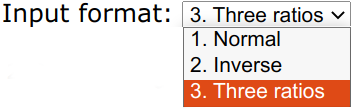
\includegraphics[width=\linewidth]{../figures/PbPbFormats.png}
\end{minipage}
\noindent\begin{minipage}[t]{.15\linewidth}
\strut\vspace*{-\baselineskip}\newline
\includegraphics[width=\linewidth]{../figures/PbPbPlotdevices.png}\\
\end{minipage}
\begin{minipage}[t]{.55\textwidth}
  \texttt{IsoplotR} accommodates three Th--Pb formats (see
  Section~\ref{sec:ThPb} for details), which can be analysed by the
  same six functions as the Pb--Pb data that were discussed
  previously.
\end{minipage}

\noindent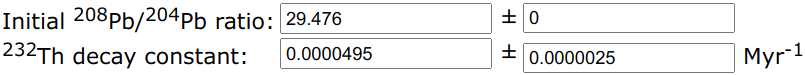
\includegraphics[width=.7\linewidth]{../figures/ThPbLambda.png}\\
\noindent The default Th decay constant is given by \citet{leroux1963}.

\begin{script}
# round the 232Th decay constant to 0.00005 +/- 0.000003
settings('lambda','Th232',0.00005,0.000003) 
\end{script}

Isochron regression proceeds in exactly the same fashion as the
generic regression function of Section~\ref{sec:OtherRegression},
apart from just two small geochronology-specific differences:

\noindent\begin{minipage}[t]{.3\linewidth}
\strut\vspace*{-\baselineskip}\newline

\includegraphics[width=\linewidth]{../figures/ThPbInverseExterr.png}
\end{minipage}
\begin{minipage}[t]{.7\
Both conventional and inverse isochrons are available, and the
analytical uncertainty of the resulting ages may be augmented by the
decay constant uncertainties.
\end{minipage}

Example of Th--Pb inverse isochron regression with error ellipses
marked by aliquot number, and empty colour ellipses with transparent
blue stroke colour:

\begin{script}
isochron(ThPb,inverse=TRUE,show.numbers=TRUE,
         ellipse.fill=NA,ellipse.stroke=rgb(0,0,1,0.5))
\end{script}

\noindent\begin{minipage}[t]{.3\linewidth}
\strut\vspace*{-\baselineskip}\newline
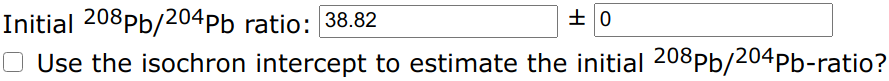
\includegraphics[width=\linewidth]{../figures/ThPbAgePb0.png}
\end{minipage}
\begin{minipage}[t]{.7\linewidth}
\end{minipage}

\noindent\begin{minipage}[t]{.5\linewidth}
\strut\vspace*{-\baselineskip}\newline

\includegraphics[width=\linewidth]{../figures/ThPbAgei2i.png}
\end{minipage}
\begin{minipage}[t]{.5\linewidth}
\end{minipage}

\section{Radial, weighted mean, KDE and CAD plots}\label{sec:PbPbOtherPlots}

\noindent\begin{minipage}[t]{.45\linewidth}
\strut\vspace*{-\baselineskip}\newline
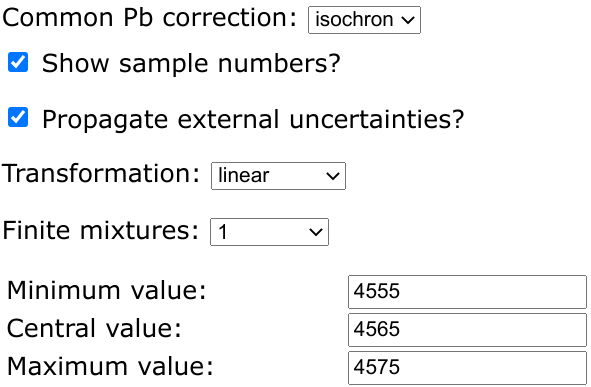
\includegraphics[width=\linewidth]{../figures/PbPbRadialOptions.png}
\end{minipage}
\begin{minipage}[t]{.55\linewidth}
  Apart from a possible common Pb-correction, the radial plot options
  for Pb--Pb data are exactly the same as for the generic radial plot
  function of Section~\ref{sec:OtherRadial}. Thus, the aliquots can be
  numbered; decay constant uncertainties may or may not be added to
  the standard error of the central age; the user can choose between
  the logarithmic, linear and square root transformations; the extent
  of the radial scale can be modified; etc.
\end{minipage}

\begin{console}
radialplot(PbPb,show.numbers=TRUE,exterr=TRUE,transformation='linear',
           k=1,from=4555,to=4575,z0=4565)
\end{console}

Similarly, the weighted mean, KDE and CAD functions work exactly as
the generic versions of Chapter~\ref{ch:generic-R}, with the only
difference being the common Pb correction, and the ability to
propagate external uncertainties.\\

\noindent CLI examples:

\begin{enumerate}

\item The weighted mean using a nominal common Pb correction with
  \textsuperscript{206}Pb/\textsuperscript{204}Pb = 9.15 and
  \textsuperscript{207}Pb/\textsuperscript{204}Pb = 10.23; applying
  the random effects model and plotting the ranked ages:
  
\begin{script}
settings('iratio','Pb206Pb204',9.15)
settings('iratio','Pb206Pb204',10.23)
weightedmean(PbPb,common.Pb=1,random.effects=TRUE,ranked=TRUE)
\end{script}

\item An orange KDE without histogram or rug plot, using an isochron
  based common Pb correction, with a 20~Myr bandwidth and axis limits
  from 4500 to 4600~Ga:

\begin{console}
kde(PbPb,kde.col='orange',rug=FALSE,show.hist=FALSE,
    common.Pb=2,bw=20,from=4500,to=4600)
\end{console}

\item a CAD with without vertical lines and steps marked by `x':

\begin{console}
cad(PbPb,verticals=TRUE,pch='x')
\end{console}
  
\end{enumerate}

\printbibliography[heading=subbibliography]

\end{refsection}
